\section{Einflussfaktoren}

Wir haben die wichtigsten Einflussfaktoren, die wir für unsere Unternehmung berücksichtigen müssen, gesammelt und stellen diese in Abbildung \ref{fig:Einflussfaktoren} grafisch dar.
	
\begin{figure}[H]
\centering
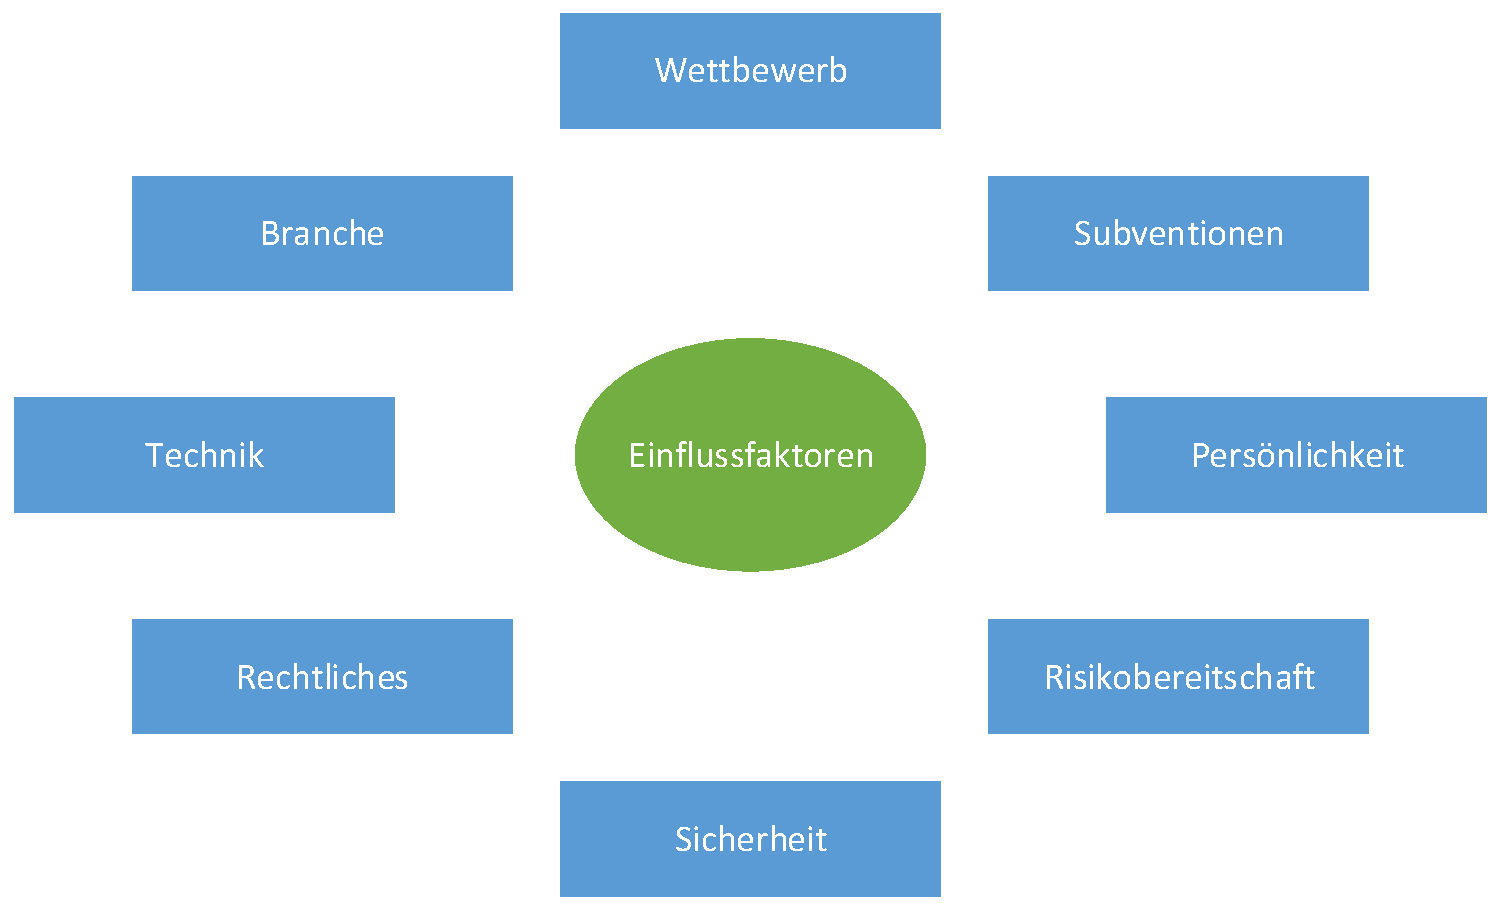
\includegraphics[width=1.0\linewidth]{Bilder/Einflussfaktoren}
\caption{Einflussfaktoren auf unsere Dienstleistung}
\label{fig:Einflussfaktoren}
\end{figure}

\begin{description}
\item[Wettbewerb:]{Der Wettbewerb beschreibt die Marktsituation. Der Markt könnte schnell gesättigt sein, so dass für uns eine Selbständigkeit nicht in Frage käme. }

\item[Subventionen]{Die Bundesregierung subventioniert Industrie 4.0 Anwendungen in ihrer Digitalisierungsoffensive, was unseren potentiellen Kunden den Vorteil verschafft, mit geringerer Eigeninvestition den Sprung in die Zukunft zu schaffen. Für uns bedeutet das eine bessere Auftragslage.}

\item[Persönlichkeit]{Unsere Persönlichkeit stellt einen wichtigen Einflussfaktor auf eine mögliche Selbstständigkeit dar. Bei fehlender Arbeitsbereitschaft und mangelndem Mut ist eine Selbstständigkeit meist von Vornherein zum Scheitern verurteilt.}

\item[Risikobereitschaft]{Die Bereitschaft eines Endkunden zu riskieren, dass eine Anlage unvorhergesehen ausfällt und die Produktion stoppt, ist für uns äußerst wichtig. Einem Kunden, dem alles egal ist, werden wir keine Predictive Maintenance Lösung verkaufen können.}

\item[Sicherheit]{Die Sicherheit von Daten und Anlagen hat höchste Priorität. Eine laufende Produktionsanlage ans Internet anzubinden, muss den höchsten Sicherheitsstandards genügen. Die Möglichkeiten sowie die Bedrohungen stellen einen Einflussfaktor für uns dar.}

\item[Rechtliches]{Die rechtliche Entwicklung im Umgang mit Anlagendaten bzgl. Datenschutz und Verantwortlichkeiten beeinflussen unsere Lösungen ggf. entscheidend.}

\item[Technik]{Die aktuell vorhandene sowie zukünftig verfügbare Technik ist einer unserer bedeutendsten Einflussfaktoren. Lösungen für die Verwaltung von Big Data und dessen Auswertung ist ebenso bedeutend wie einsetzbare Sensorik.}

\item[Branche]{Die Branche beeinflusst uns z.B. bei der Standortauswahl oder Ergebnisdefinition in Form von Ofenzuverlässigkeit.}
\end{description}

